\section{Technologies}

% This is a comment

In order for autonomous vehicles (AVs) to behave like any other car, technologies employed must be sufficiently diversified and advanced to reproduce the human cycle of sense, decide, and act using sensors, algorithms and mechanics.

\begin{center}
    \begin{figure}[ht!]
        \centering
        
        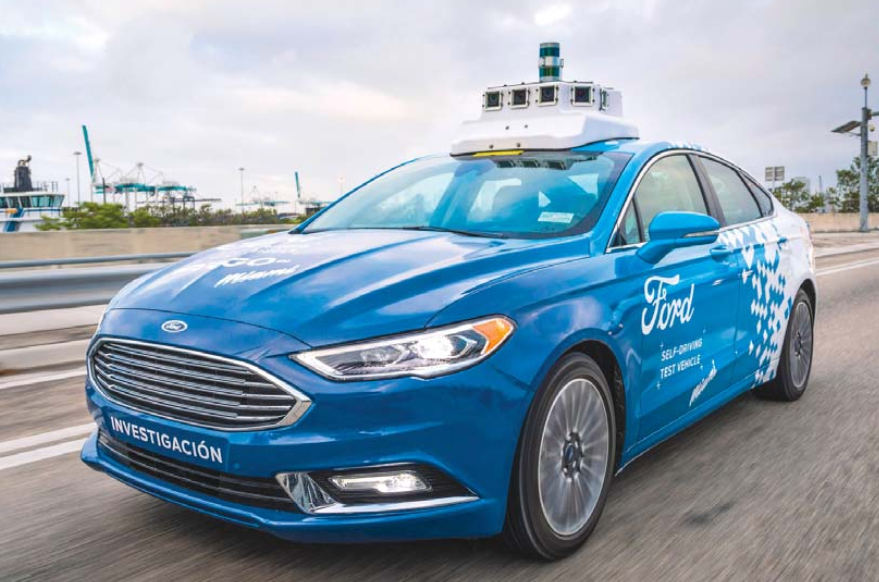
\includegraphics[width=467px, keepaspectratio]{imports/autonomous_vehicle.png}
        
        \caption{an example of an autonomous vehicle, the Ford Argo}  \cite{mccormick_self-driving_2019}
    \end{figure}
\end{center}

\subsection{Sensors for the autonomous vehicle}

To be aware of its environment, an AV usually carries a big cumbersome sensor package, because, to be sure the vehicle will not miss any detail in its environment, sensors redundancy and diversity are fundamental.

\subsubsection{LiDAR}

Out of all of the sensors, LiDAR is the most important and expensive, it costs tens of thousands of dollars. It is composed of an array of semiconductor lasers and optical detectors mounted on a rotating platform in an enclosure. By emitting pulses of near-IR light and measuring the return time of reflections, the system calculates a point cloud of objects surrounding the vehicle.”\cite{mccormick_self-driving_2019} The image created is updated 10 times per second and locates objects in a range of 50-100m with a 2 cm precision.
\smallskip

Nowadays, most companies (except Tesla) who are developing self-driving cars use LiDARs, despite of their high cost, their precision is crucial for the vehicle to picture and reconstruct its environment.
\smallskip

“As the single most expensive [AV] component, LiDAR has been the focus of intense R\&D by industry.”\cite{mccormick_self-driving_2019} Today, they are interested in replacing its rotative architecture that is cause of failure. Different approaches are being taken like using electromechanical mirrors for example, they intend to “steer laser beams without bulk mechanical motion”\cite{mccormick_self-driving_2019} and might allow to focus beams on detected objects to acquire more information about them.
\smallskip

Another preoccupation about LiDARs is eye safety, wavelengths used by LiDARs (900 nm) are quite dangerous for retina so, for now, power is limited. LiDARs with a higher, safer, wavelength exist but they require very expensive rare metals.

\subsubsection{Radar}

However, LiDARs can be easily limited by bad weather conditions and are relatively short-ranged. Consequently, AVs also use radars ; radars can determine objects speed towards the car (thanks to Dopler shift) allowing the AV to detect pedestrians and other vehicles. Furthermore, radars are cheaper (they cost hundreds of dollars) than LiDAR and still work in poor weather conditions.

\smallskip
AVs combine LiDAR and radar data for two tasks. It determines position and orientation in space with more precision than the GPS by locating landmarks on a base map. It also identifies and tracks moving objects ; their position and speed are then determined using statistical algorithms. The main inconvenient of the first task is the high dependence to already existing highly detailed maps.

\subsubsection{Camera}

The last sensor used by AVs is camera. Cameras with different focuses are used (near, far). Images are then analysed by neural networks to detect and classify objects including spotlights, lines, streets signs, etc. These data are used to validate or cancel trajectories calculated from the LiDAR and radar data.

\subsubsection{Sonar}

Until recently, ultrasonic sensors (sonars) were limited to parking assist because of their limited range, but, long range sonars exist nowadays. As a result, researchers developed an AV using a long-range ultrasonic sensors system\cite{budisusila_review_2019} capable of adapting to the speed of the vehicle, and braking if objects are detected on its trajectory albeit considering the distance between the vehicle and other vehicles behind the it. Ultrasonic sensors also have the advantage to be cheap, easy to implement in most vehicles, and calculations to get range information of the detected object are simple.

\subsection{Algorithms and control systems}

AVs carry sensors in order to get information about their environment, but these raw data must be analysed and treated to ensure the vehicle reacts accordingly. They need especially a path planning algorithms to find the best path to their destination, and to take into account detected objects like pedestrians that might be on it.

\subsubsection{Path planning}

Path planning uses all the data retrieved by the previously presented sensors, it includes two levels: a strategic level (the higher one) that decides, for example, if the car should overtake another car or wait, and a tactical level (the lower one) that determines, for example, the optimal steering angle or speed needed to accomplish an optimal maneuver.
\smallskip

Sensors work at a higher rate than path planning. Path planning is done on board the vehicle because the vehicle needs the best reaction time.
\smallskip

GPU are used to maximize the processing speed because most calculations are similar and can be parallelized. They are also used to train neural networks with data collected by vehicles.

\subsubsection{Pedestrian detection}

A challenge is to detect the pedestrians, for example, crossing or walking along the road. Indeed, it is a moving target and it can behave unexpectedly, becoming a danger. A way to predict the move of a pedestrian is to only use detection i.e consider it as an object in front of the vehicle,  and then react. But another way has been researched \cite{sarcinelli_handling_2019}, the path tracking of pedestrian. The latter is better in decision making and provides a more efficient and safer driving experience.

\begin{center}
    \begin{figure}[ht!]
        \centering
        
        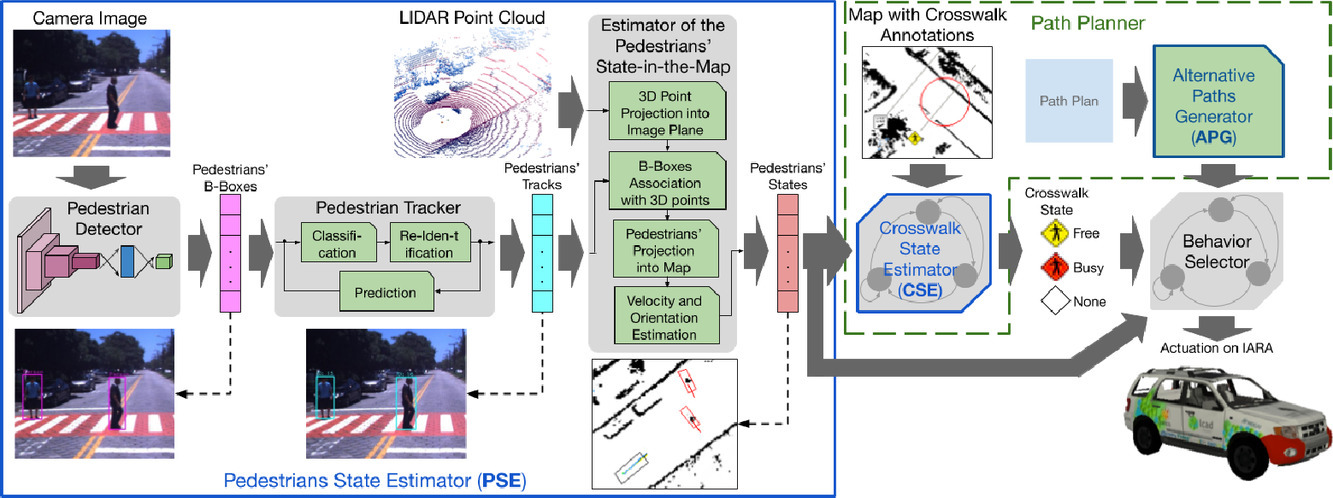
\includegraphics[width=467px, keepaspectratio]{imports/pedestrian1.jpg}
        
        \caption{Overview of the autonomous pedestrian detection architecture}  \cite{sarcinelli_handling_2019}
    \end{figure}
\end{center}

This technology allows to use temporal information for keeping track of the state (position, velocity, and orientation) of pedestrians, which allows the prediction of the near-future pedestrians' states (~3–5 s ahead).
\smallskip
The technology is divided in two main parts: the Perception System and the Decision-Making system. The first one is responsible for tasks of localizing the self-driving car, mapping of obstacles,tracking of moving obstacles, and recognition of traffic signalization. The second one is responsible for correctly driving the car according to the information provided by the perception system i.e control, path planning, behavior selection. 

\smallskip
In order to diminish the use of the Decision-Making part, many useful tasks to pedestrian detection are already performed at detection. The pedestrian boxes are calculated using a Convolutional Neural Network (CNN) in order to reduce the computational overhead, that is useful, considering that the detection of pedestrian is not the only computing that an autonomous car has to perform. For instance, YOLOv3 CNN \cite{redmon_yolov3:_2018} is one of the state-of-the-art systems for real-time object detection that is based on a bounding box (B-Box) regression, and include the Pedestrians’ Tracks which mainly classifies bounding-boxes of people present in scene as new or previously tracked person as seen in the figure 2.
\begin{center}
    \begin{figure}[ht!]
        \centering
        
        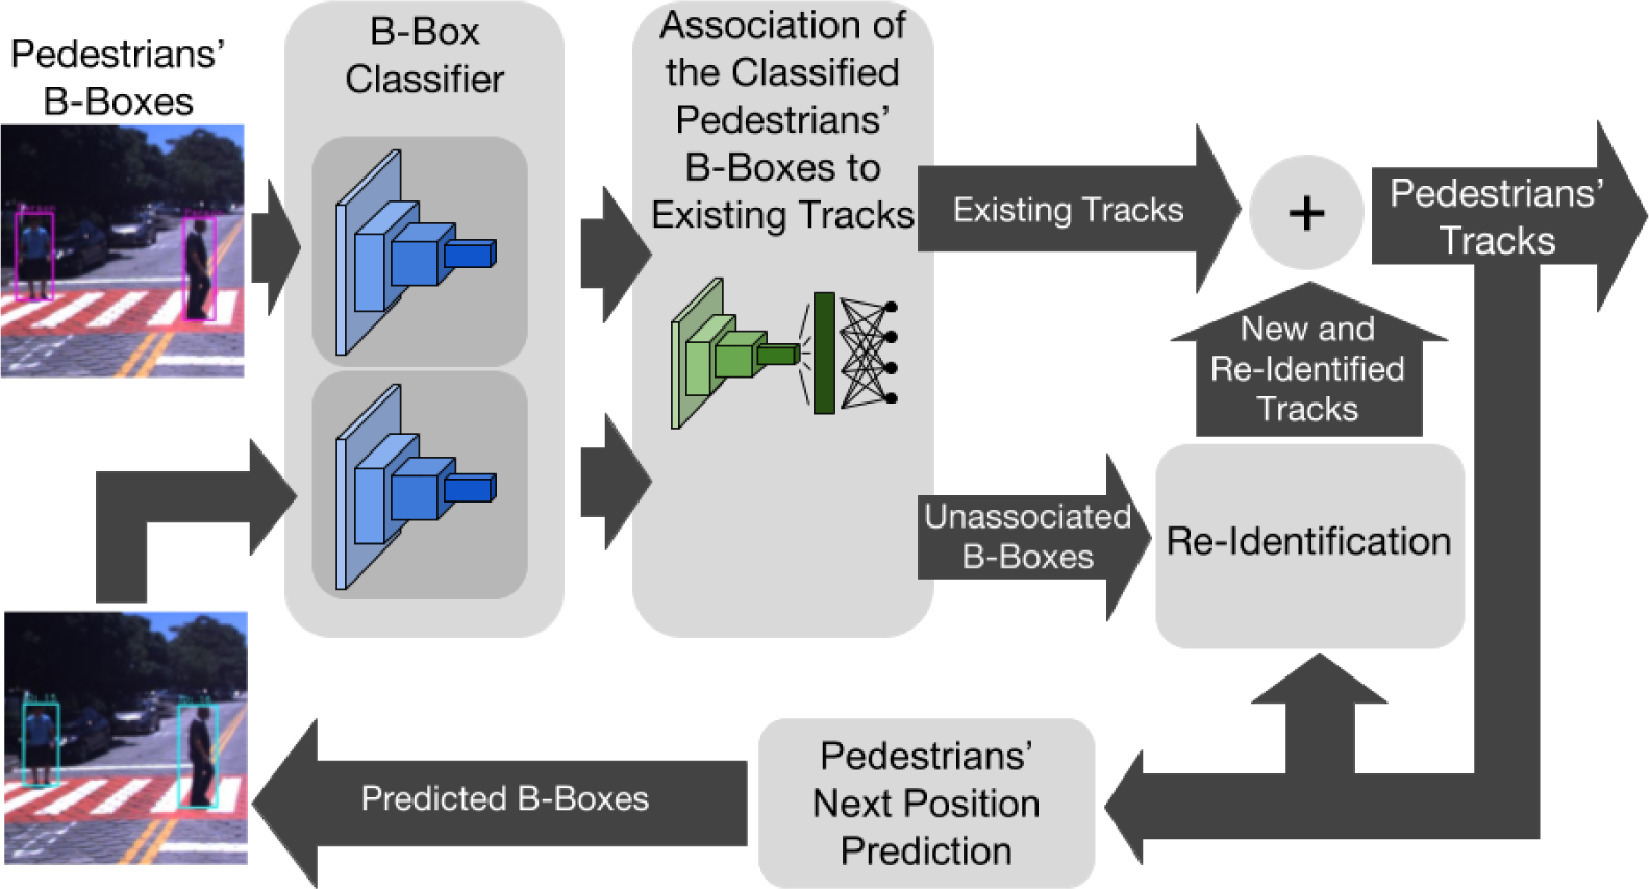
\includegraphics[width=467px, keepaspectratio]{imports/pedestrian2.jpg}
              \caption{Overview of the tracking system}
              \cite{sarcinelli_handling_2019}
    \end{figure}
\end{center}
First of all, the pedestrian boxes retrieves the camera picture from CCN, then we use LiDAR to get their position information in 3D, velocity and the accuracy of camera’s information (by providing others physics information) \cite{guidolini_handling_2018}. Pedestrians’ State-in-the-Map Estimator is the one who centralise all the LiDAR. It projects those 3D points collected by LiDAR into images, then calculate their real position by referencing the coordinate of the pedestrian boxes placed and the distance of the vehicle estimated , and finally provide a vector of triplets (position, orientation,velocity) to the decision making system to act accordingly.  
\smallskip

Finally, in the decision making part, the Crosswalk State Estimator (CSE) predicates the near future behaviour i.e whether the crosswalk is busy (has one or more pedestrians demanding right of passage) or free.
To perform that, the system is based on the car's velocity, the distance between the car and the crosswalk, and the presence of pedestrians around the crosswalk area and their walking speed/direction.
A state machine is used to predicate the pedestrians' intentions. To sum up,  intention exists if, and only if, the pedestrian is moving in the approximate direction (+/-30 degrees) of the center of the crosswalk area or is inside a crosswalk area and in the car’s path or  if velocity is equal or greater than 0.3 m/s and the pedestrian is not moving in the approximate direction (+/-30 degrees) of the road, meaning that he will perhaps cross the road soon. The angle range in both presented scenarios were empirically defined considering a normal human behaviour on these situations \cite{sarcinelli_handling_2019}.

There are a lot of methods to build an AV, on both hardware level and software level. Concerning the hardware, microprocessors/controllers units having GPIO ports (like arduino or raspberry pi) are used in recent studies. About the software, many algorithms are used like PID, fuzzy logic inference, and genetic algorithms, but the usage of neural network algorithms is quite rare.

\subsubsection{ADAS (Advanced Driver Assistant System)}

The ADAS is used in semi-automatic cars, unlike the systems found in AVs, its goal is not to replace the driver, but to turn it into an observer who monitors the movement of the car.

\subsubsection{Ultrasonic sensor system}

In 2004, a team designed "an ultrasonic sensor system to prevent accidents on the sides of the vehicle."\cite{budisusila_review_2019} The system was designed to be used in town at a speed of around 40 km/h, and sensors had a 6 meters range.

\subsubsection{ACC (Adaptive Cruise Control)}

The ACC system is used for longitudinal control of the vehicle (acceleration and deceleration), it takes three inputs:
\begin{itemize}
    \item Vehicle speed
    \item Driver setting time
    \item Distance measured by sensors (radars, sonars)
\end{itemize}
For an AV to follow another vehicle and stay at a reasonable distance, a new reference speed is calculated by the controller in a loop.